\usetikzlibrary{arrows,shapes,chains}
\section{First section}
\frame
{
  \frametitle{\secname~ }
  \begin{columns}[onlytextwidth]
  \begin{column}{0.35\textwidth}
  \begin{block}{plan}
  \begin{itemize}
    \item xxxxx
    \item xxxxxx
    \item xxxxx
  \end{itemize}
  \end{block}
  \end{column}
  \hspace{0.5em}
  \begin{column}{0.65\textwidth}
    \begin{block}{do}
      \begin{itemize}
        \item xxxx
        \item xxxx
        \item xxxx
      \end{itemize}
    \end{block}
  \end{column}
  \end{columns}
  \note{
    note
  }
}

\subsection{sub-section}
\frame{ 
  \frametitle{sub-section xxxxx}
  \begin{figure}  
  \tikzstyle{format}=[rectangle,draw,thin,fill=white]  
  %定义语句块的颜色,形状和边
  \tikzstyle{test}=[diamond,aspect=2,draw,thin]  
  %定义条件块的形状,颜色
  \tikzstyle{point}=[coordinate,on grid,]  
  %像素点,用于连接转移线
  \begin{tikzpicture}
    %[node distance=10mm,auto,>=latex',thin,start chain=going below,every join/.style={norm},] 
  %start chain=going below指明了流程图的默认方向,node distance=8mm则指明了默认的node距离。这些可以在定义node的时候更改,比如说 
  %\node[point,right of=n3,node distance=10mm] (p0){};  
  %这里声明了node p0,它在node n3 的右边,距离是10mm。
  	%\node[format] (n0) at(4,4){A}; 直接指定位置 
		%定义完node之后进行连线,
		%\draw[->] (n0.south) -- (n1); 带箭头实线
		%\draw[-] (n0.south) -- (n1); 不带箭头实线
		%\draw[<->] (n0.south) -- (n1.north);   双箭头
		%\draw[<-,dashed] (n1.south) -- (n2.north); 带箭头虚线 
		%\draw[<-] (n0.south) to node{Yes} (n1.north);  带字,字在箭头方向右边
		%\draw[->] (n1.north) to node{Yes} (n0.south);  带字,字在箭头方向左边
		%\draw[->] (n1.north) to[out=60,in=300] node{Yes} (n0.south);  曲线
		%\draw[->,draw=red](n2)--(n1);  带颜色的线
  \node[format] (start){aaa};
  \node[format,below of=start,node distance=10mm] (define){bbbb};
  \node[format,below of=define,node distance=10mm] (PCFinit){cccc};
  \node[format,below of=PCFinit,node distance=10mm] (DS18init){dddd};
  \node[format,below of=DS18init,node distance=10mm] (LCDinit){eeee};
  \node[format,below of=LCDinit,node distance=10mm] (processtime){ffff};
  \draw[->] (start)--(define);
  \draw[->] (define)--(PCFinit);
  \draw[->](PCFinit)--(DS18init);
  \draw[->](DS18init)--(LCDinit);
  \draw[->](LCDinit)--(processtime);
\end{tikzpicture}  
\end{figure} 
%%%%%%%%%%%%%%%%%%----------批量插入图片------------%%%%%%%%%%%%%
  % \begin{figure}
  %   \hspace{-2.0em}
  %   \begin{minipage}{1.06\textwidth}
  %     \subfloat[\scriptsize AABB]
  %     {
  %       \includegraphics[width=0.2\textwidth]{figures/bunny-2d-AABB.eps}
  %     }
  %     \subfloat[\scriptsize OBB]
  %     {
  %       \includegraphics[width=0.2\textwidth]{figures/bunny-2d-OBB.eps}
  %     }
  %     \subfloat[\scriptsize Sphere]
  %     {
  %       \includegraphics[width=0.2\textwidth]{figures/bunny-2d-Sphere.eps}
  %     }%\linebreak
  %     \subfloat[\scriptsize $k$-DOP]
  %     {
  %       \includegraphics[width=0.2\textwidth]{figures/bunny-2d-8DOP.eps}
  %     }
  %     \subfloat[\scriptsize 凸包]
  %     {
  %       \includegraphics[width=0.2\textwidth]{figures/bunny-2d-Convexhull.eps}
  %     }
  %   \end{minipage}
  %   \caption{不同种类的包围体}
  %   \label{chart:exps:tightness}
  % \end{figure}
  % \vspace{-1em}
  % 其他:Tribox、Swept-sphere、 Sphere-shell、Zonotopes、圆柱形、圆锥、椭球形等等。

  \note{
    what you prepare to say.
  }
}

\frame{
  \frametitle{frame title}
  \footnotesize
  %\textbf  加粗
  acacacacacacacacacaccacacacacacaca
  \begin{block}{plan}
    \hspace{-2.0em}   \begin{minipage}{\textwidth}
      \begin{description}
        \item[item1] aaaa
        \item[item2] bbbb\\
                     cccc
        \item[item3] dddd
      \end{description}
    \end{minipage}
  \end{block}

  \note{
    What you say by your mouth

  }
}

\subsection{latex}
\frame{
  \frametitle{\subsecname~ }
  \begin{figure}[htb]   
    \center{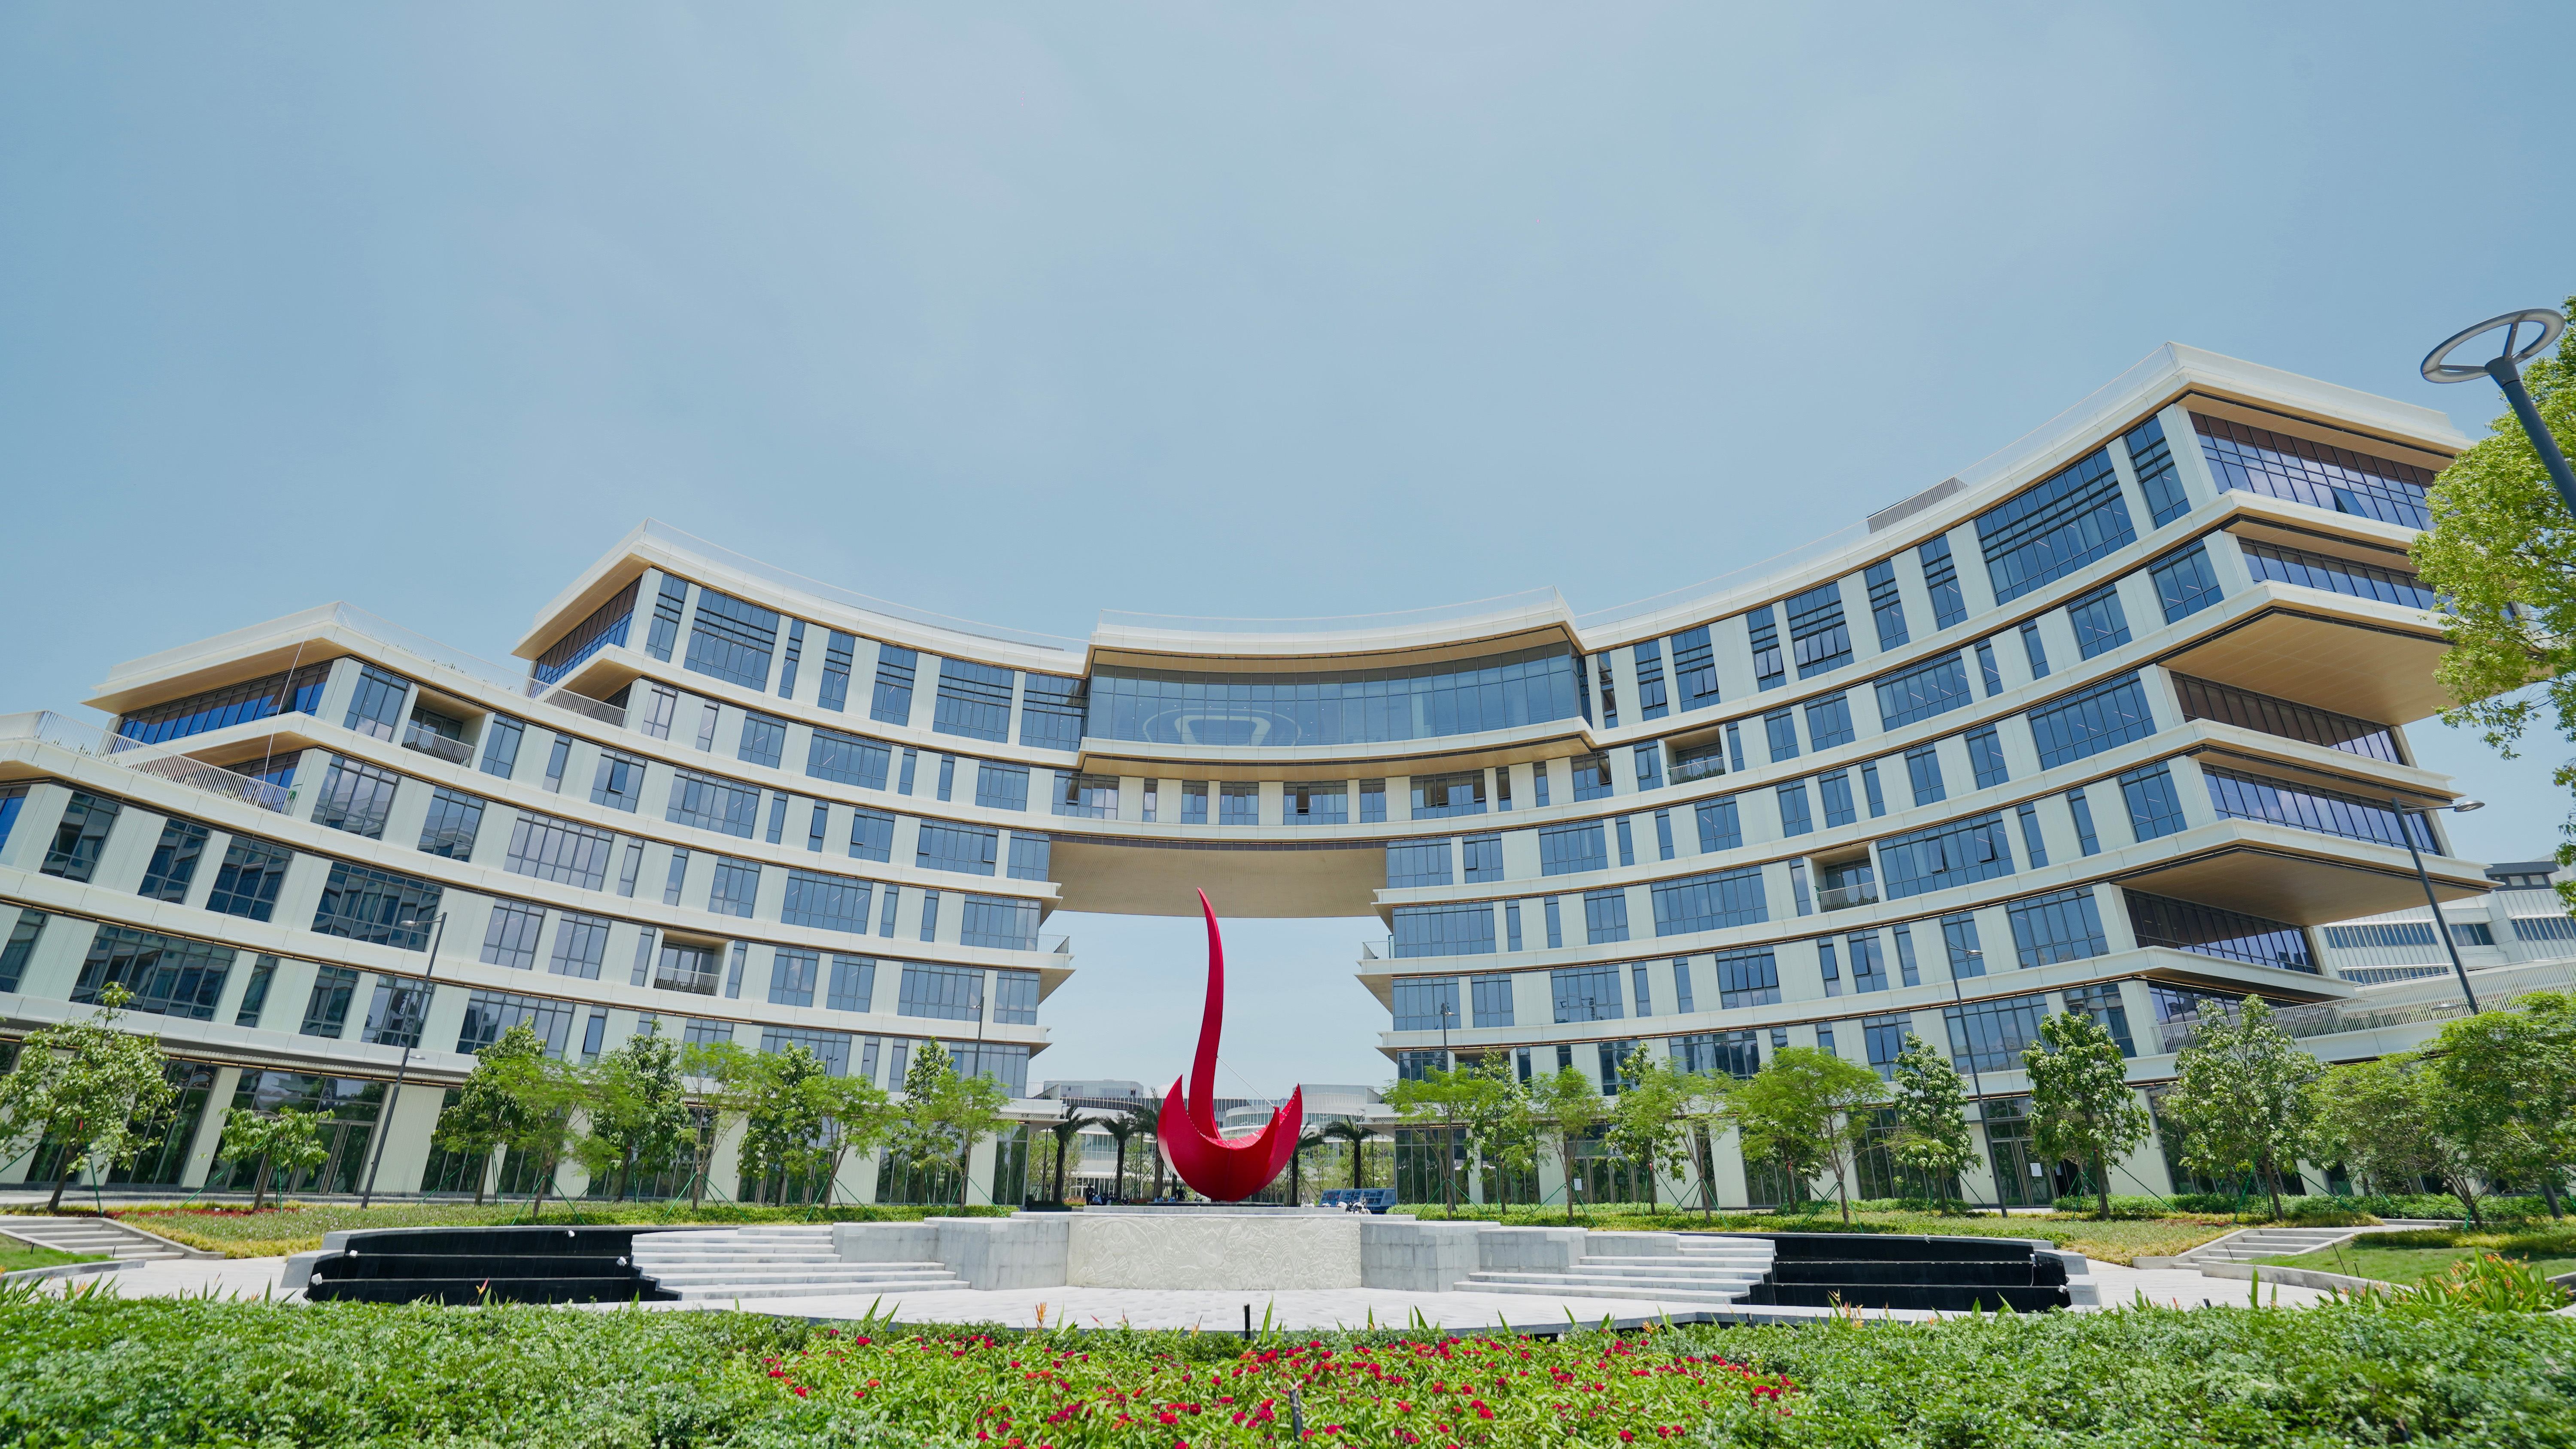
\includegraphics[width=8cm]  {figures/home_bg_1.jpg}}   
    \caption{\label{1} figure 1}    
  \end{figure}


  \note{
    (介绍PPT后)
  }
}

% \frame{
%   \frametitle{基于~BVH~的碰撞检测算法}
%   \begin{columns}[onlytextwidth]
%     \begin{column}{0.35\textwidth}
%       \vspace{-1.5em}
%       \begin{figure}[htbp]
%         \begin{center}
%           \begin{boxedminipage}{1\textwidth}
%             \subfloat{\label{lbl:bvh-bunny-center-0.png}}
%             {\includegraphics[height=1.4cm]{bvh-bunny-center-0.png}}
%             \subfloat{\label{lbl:bvh-bunny-center-1.png}}
%             {\includegraphics[height=1.4cm]{bvh-bunny-center-1.png}}
%             \\
%             \subfloat{\label{lbl:bvh-bunny-center-2.png}}
%             {\includegraphics[height=1.4cm]{bvh-bunny-center-2.png}}
%             \subfloat{\label{lbl:bvh-bunny-center-3.png}}
%             {\includegraphics[height=1.4cm]{bvh-bunny-center-3.png}}
%             \\\hspace{0.5cm}
%             \subfloat{\label{lbl:bvh-bunny-center-4.png}}
%             {\includegraphics[height=1.5cm]{bvh-bunny-center-4.png}}
%             \subfloat{\label{lbl:bvh-bunny-center-5.png}}
%             {\includegraphics[height=1.5cm]{bvh-bunny-center-5.png}}
%             \\
%             \subfloat{\label{lbl:bvh-bunny-center-6.png}}
%             {\includegraphics[height=1.5cm]{bvh-bunny-center-6.png}}
%             \subfloat{\label{lbl:bvh-bunny-center-7.png}}
%             {\includegraphics[height=1.5cm]{bvh-bunny-center-7.png}}
%           \end{boxedminipage}
%           \vspace{-0.5em}
%           \caption{八层~BVH~示例}
%           \label{lbl:bvh-example}
%         \end{center}
%       \end{figure}
%     \end{column}
%     \hspace{0.5em}
%     \begin{column}{1.2\textwidth}
%       \vspace{0.2em}
%       \scalebox{0.5}{
%         \begin{minipage}{1.0\textwidth}
%           \vspace{-2em}
%           \begin{algorithm}[H]
%             \caption{自顶向下层次遍历~BVH~}
%             \label{alg:traverse-bvh-tree}
%             \begin{algorithmic}[1]
%               \Require
%               两个~BVH~树的根节点~$node_1$,$node_2$
%               \Ensure
%               模型是否相交
%               \Function {TraverseBVHTree}{$node_1, node_2$}
%               \If{$node_1.bv \cap node_2.bv = \emptyset$}
%               \State \Return{\textbf{False}}
%               \Comment{包围体重合测试, 包围体不相交直接返回}
%               \Else
%               \If {$node_1.children = \emptyset$}
%               \If {$node_2.children = \emptyset$}
%               \State \Comment{最底层叶子节点原生几何相交测试}
%               \State \Return {\Call{CheckIntersection}{$node_1.primitives, node_2.primitives$}}
%               \Else
%               \ForAll {$child \in node_2.children$}
%               \State \Call{TraverseBVHTree}{$node_1, child$} \Comment{递归调用}
%               \EndFor
%               \EndIf
%               \Else
%               \ForAll {$child \in node_1.children$}
%               \State \Call{TraverseBVHTree}{$child, node_2$}  \Comment{递归调用}
%               \EndFor
%               \EndIf
%               \EndIf
%               \EndFunction
%             \end{algorithmic}
%           \end{algorithm}
%         \end{minipage}
%       }
%       \\
%       \scriptsize \hspace{1em}代价函数: $T_{cost} = n_v * C_v + n_p * C_p + (n_u * C_u)$(运动)
%     \end{column}
%   \end{columns}
%   \note{
%     基于包围体树的碰撞检测算法, 一般首先都会初始化环境然后构建层次结构的包围体树,碰撞检测时从顶层开始逐渐往下层遍历,到最底层叶子节点后开始三角网格模型相交测试,
%     当发现三角网格相交后立即终止遍历,确定模型发生碰撞。
%     评价碰撞检测算法的指标一般用上面这个公式来衡量,其中nv和 np分别表示参与包围体节点相交测试的数量和参与原始几何相交测试的数量,Cv和 Cp则表示相应的平均测试耗费的代价。
%     当在运动场景时还需要加上nu和 Cn就是模型旋转或者运动后包围体更新的数量和更新的代价。
%     本文算法就是尽早发现包围体不相交的情况,减少np和cp的数量。
%   }
% }
